\documentclass[tikz,border=10pt]{standalone}
\usepackage{tikz}
\usetikzlibrary{arrows.meta,arrows}
\usepackage{amsmath}
\usepackage{physics}

\ExplSyntaxOn
\msg_redirect_name:nnn { siunitx } { physics-pkg } { none }
\ExplSyntaxOff

\begin{document}


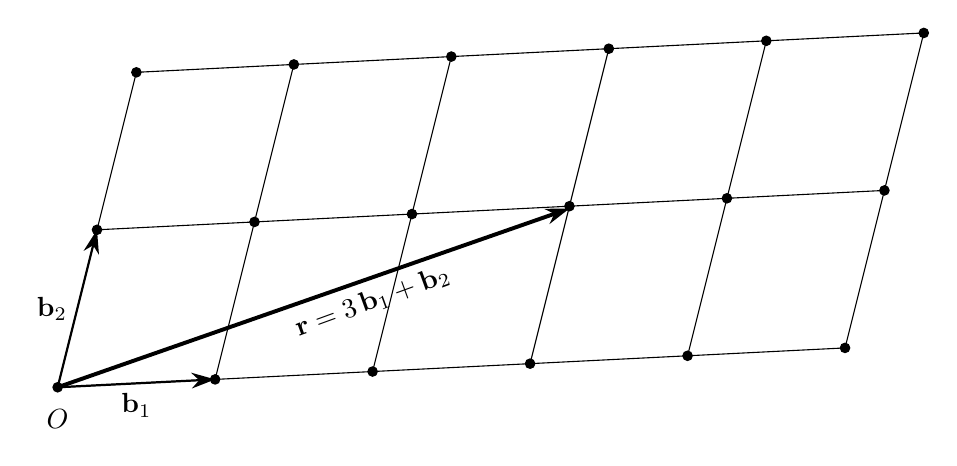
\begin{tikzpicture}[scale=2]
    \node at (0, -0.2) {$O$};
    \draw (0, 0) -- (5, 0.25);
    \draw (0, 0) -- (0.5, 2);
    \draw (5, 0.25) -- (5.5, 2.25);

    \draw (0.25, 1) -- (5.25, 1.25);
    \draw (0.5, 2) -- (5.5, 2.25);

    \foreach \x in {1, 2, 3, 4}
        \draw (\x, \x*0.05) -- (\x+0.5, 2+\x*0.05);

    \foreach \x in {0, 1, 2, 3, 4, 5}
    {
        \draw[fill] (\x, \x*0.05) circle (0.03);
        \draw[fill] (\x+0.25, 1+\x*0.05) circle (0.03);
        \draw[fill] (\x+0.5, 2+\x*0.05) circle (0.03);
    }
    \draw [-{Stealth[length=3mm, width=2mm]}, thick] (0, 0) -- (0.25, 1) node[midway, left] {$\vb{b}_2$};
    \draw [-{Stealth[length=3mm, width=2mm]}, thick] (0, 0) -- (1, 0.05) node[midway, below] {$\vb{b}_1$};
    \draw [-{Stealth[length=3mm, width=2mm]}, line width = 0.5mm] (0, 0) -- (3.25, 1.135) node [below, pos=0.6, rotate=20] {$\vb{r} = 3 \, \vb{b}_{1} + \vb{b}_{2}$};

\end{tikzpicture}
\end{document}